%%
%% $Id$
%%
%% Copyright (c) 2007-2008 Christian Fehler
%% Copyright (c) 2007-2008 Benjamin Mies
%%


\chapter{Konzepte}\label{Concepts}

In diesem Kapitel werden alle wichtigen Konzepte besprochen, die bei der
Umsetzung des \gtitools berücksichtigt bzw. erst während der Entwicklung
diskutiert und anschließend in die Tat umgesetzt wurden.\vspace{10pt}


\section{Unterstützung von Lerngruppen}\label{ConceptsLerning}

Ein wichtiges Konzept bei der Umsetzung war die Unterstützung von Lerngruppen.
Das \gtitool sollte somit in irgendeiner Weise dazu in der Lage sein, nicht nur
einem Benutzer zur Verfügung zu stehen, sondern sollte auch von einer
Lerngruppe benutzt werden können. Bei der Planung wurden verschiedene
Möglichkeiten diskutiert, auf welche Weise wir Lerngruppen unterstützen
können. Schließlich wurde beschlossen, den Benutzern einen Austausch von
geöffneten Automaten und Grammatiken zu ermöglichen.\vspace{10pt}

\begin{figure}[h!]
\begin{center}
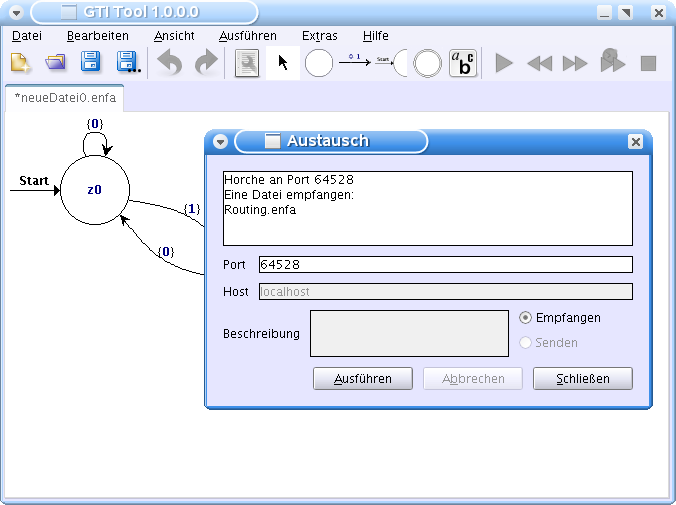
\includegraphics[width=12cm]{../images/exchange.png}
\caption{Unterstützung von Lerngruppen}
\end{center}
\end{figure}
\vspace{10pt}

Der Austausch von Dateien wurde so umgesetzt, dass ein Benutzer seine
geöffneten Dateien an andere Benutzer verschicken kann, falls der Empfänger
zuvor das Empfangen eingeleitet hat. Somit sind Mitglieder von Lerngruppen in
der Lage, Erkenntnisse mit den Anderen auszutauschen. Dies sollte dazu dienen,
das Verständnis der Materie zu verbessern.\vspace{10pt}


\section{Möglichst wenig Eingabebeschränkungen}\label{ConceptsInput}

Ein weiteres sehr wichtiges, wenn nicht sogar das wichtigste Konzept bei der
Umsetzung, war, die auch in Abschnitt \ref{InteractionErrorWarning} angesprochene
Vorgehensweise mit Benutzereingaben. Der Benutzer sollte so wenig wie möglich in
der Eingabe beschränkt werden. Ein Beispiel dafür ist, dass er in einem DEA einen
$\epsilon$-Übergang anlegen kann, obwohl dies für diesen Automaten nicht erlaubt
ist. Allerdings kann er einen solchen Automaten nicht benutzen, denn bevor etwas
ihm, zum Beispiel eine Wort-Navigation, erfolgen kann, wird der Automat
automatisch validiert, wobei die in Abschnitt \ref{InteractionErrorWarning}
angegebenen Fehler und Warnungen auftreten können.\vspace{10pt}

Hintergrund von diesem Konzept war, dass der Benutzer durch dieses Vorgehen mehr
lernt, als wenn er, um in dem Beispiel zu bleiben, einen $\epsilon$-Übergang gar
nicht erst hätte anlegen dürfen. Dann hätte er sich vermutlich nur gewundert,
warum er \Symbol{$\epsilon$} nicht der Übergangs-Menge hinzufügen
kann.\vspace{10pt}
